While cracks are actually sharp two-dimensional hypersurfaces the phase-field fracture approach
regularizes the sharp material discontinuities with smooth transitions between broken and unbroken regions. The evolution of the phase-field follows an evolution equation where the driving
forces of crack growth are derived from an energy minimization principle, typically based on
an Ambrosio-Tortorelli type functional. Modifications allow accounting for the no-healing irreversibility constraint of crack evolution and, especially important, for the asymmetry of fracture,
i.e., the fact that cracks only grow under tensile loadings but not under compression. Further
modifications consider the evolution problem at finite strains using energy densities, which are
polyconvex functions of the deformation, [1, 2].
In this contribution different decompositions of the elastic energy and the pros and cons of
variational and ad hoc formulations for the crack driving forces will be discussed. The latter
may base on positive principal stresses or strains for example. We compare different models in
linearized and in finite elasticity and present recent results on the mathematical analysis for a
phase-field model at finite strains, where we formulate the phase-field with energy densities in
terms of the modified invariants of the right Cauchy-Green strain tensor. To illustrate the capability of a phase-field fracture approach we present finite element simulations of brittle fracture
and compare it to our experimental results. The main challenge of such fracture simulations
is, that it requires the ability of a numerical method to predict crack nucleation and fracture
without stress concentration at a notch or at an initial crack.
\begin{figure}[h]
\centering
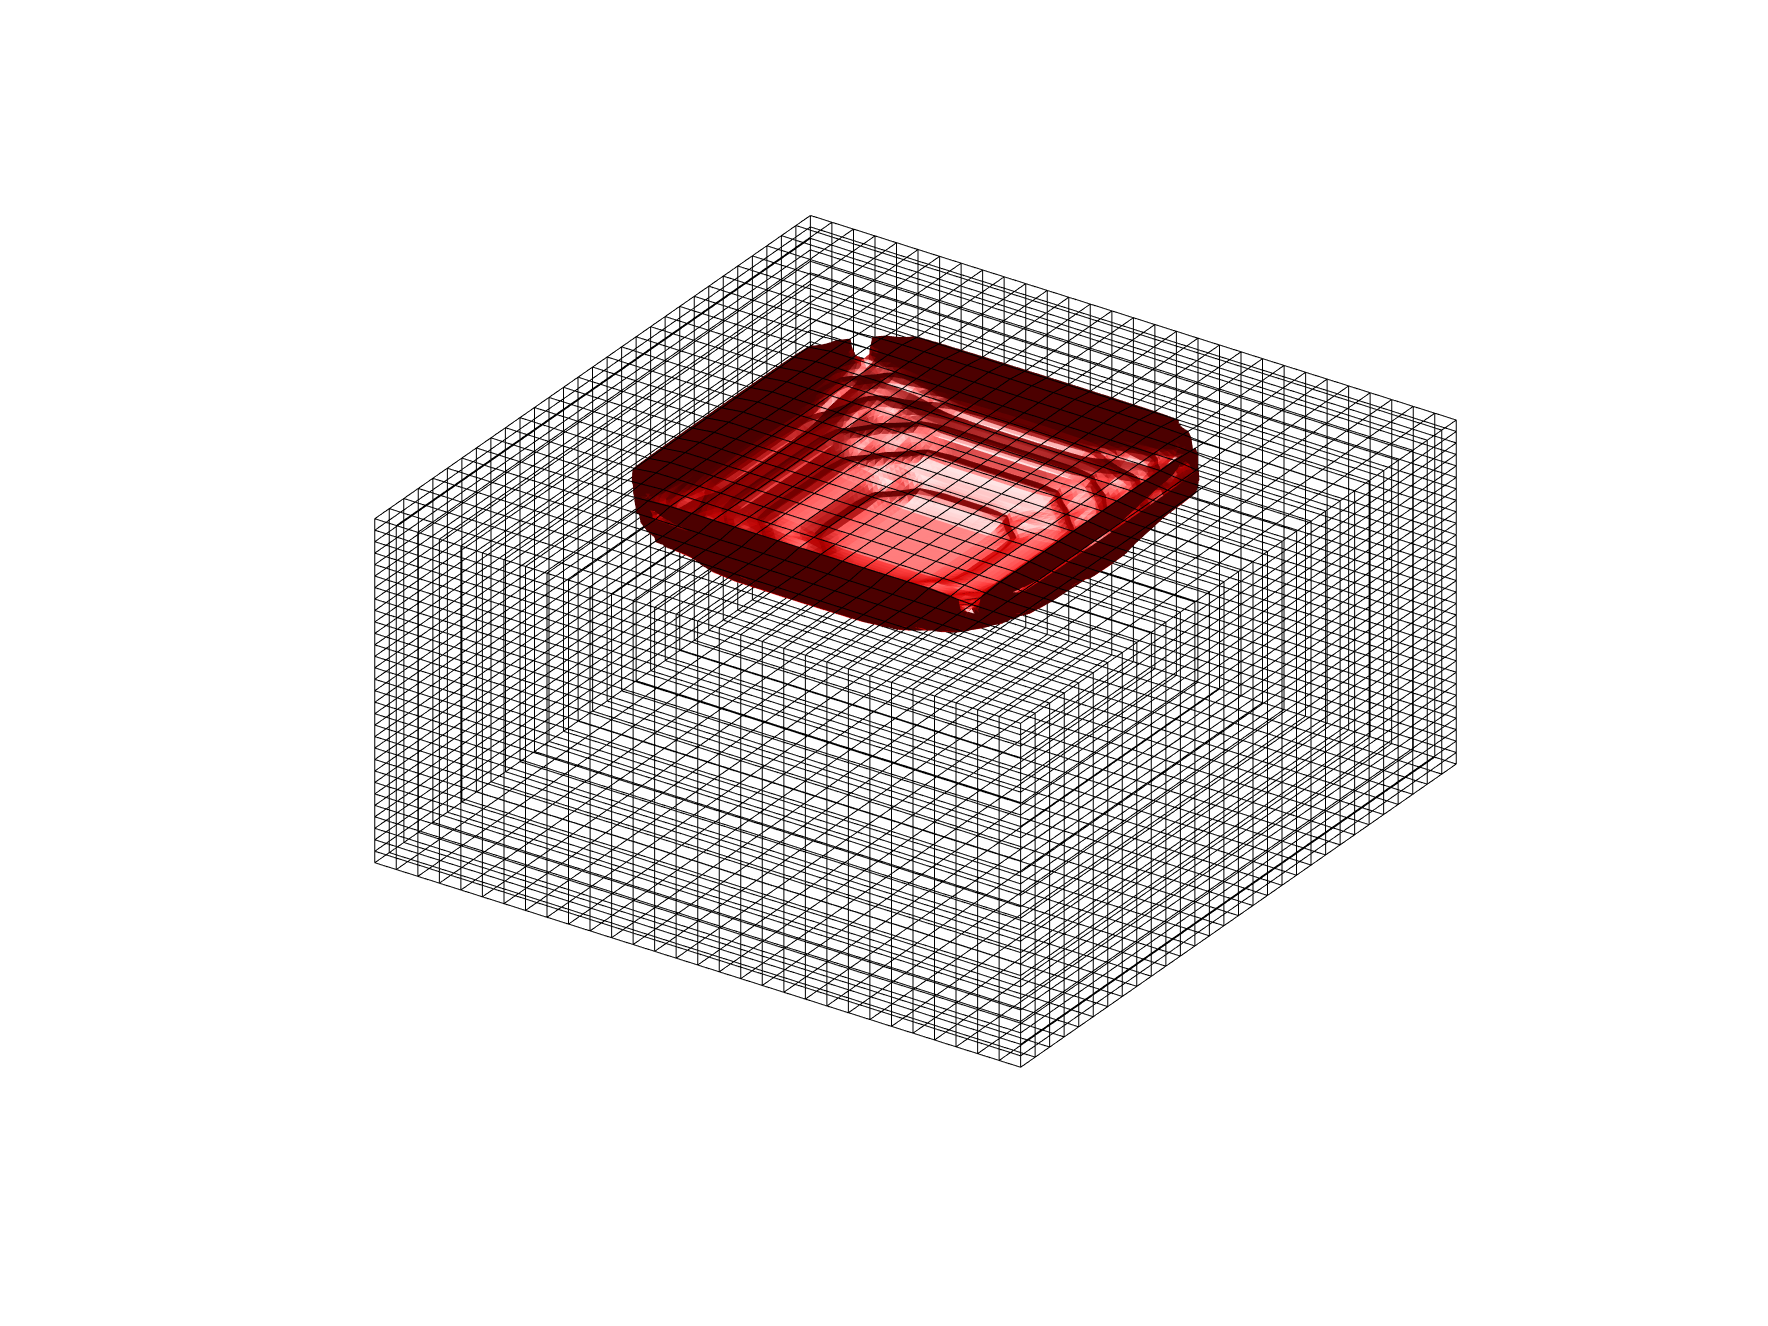
\includegraphics[width=0.4\textwidth]{data/BM3D_Yeoh_TS80_iso.png}
%\caption{Crack surface in conchoidal fracture \cite{Bilgen_etal2017}} \label{fig:crackNH_MR}
\vspace{-1cm}
\end{figure}

\noindent\textbf{References}\\
$[$1$]$ C. Bilgen, K. Weinberg. On the crack-driving force of phase-field models in linearized and
finite elasticity Comp. Meth. in Appl. Mech. and Engng, 353:348–372, 2019\\\newline
$[$2$]$ C. Bilgen, A. Kopaničáková, R. Krause, K. Weinberg. A phase-field approach to conchoidal
fracture. Meccanica, 53:1203-1219, 2018
